\section{Comparison of the Conjugate Gradient Method}\label{sec:results}
The main code used to solve the linear system using the CG and PCG methods is shown in Code \ref{code:main}. 
\begin{lstlisting}[language=Python, caption={Main code to solve the linear system using the CG and PCG methods.}, label={code:main}]{Code/main.py}
from List3.SparseMatrix import SparseMatrix
from IndirectSolver import IndirectSolver

def ParseVector(file: str)->np.array:
    with open(file, "r") as f:
        vector = np.array([float(x) for x in f.read().split(",")])      
    
    return vector

def Main()->None:
    matrix_file = "List4/matrix.dat"
    rhs_file = "List4/rhs.dat"
    results_file = "List4/Results.py"

    niter = 500

    matrix = SparseMatrix()
    matrix.ParseFromFile(matrix_file)

    rhs = ParseVector(rhs_file)

    solver = IndirectSolver(matrix, rhs, niter = niter)

    solver.Set_method("ConjugateGradient")
    solver.Solve()
    resnormCG = solver.resnorm

    solver.Set_preconditioner("Jacobi")
    solver.Solve()
    resnormCGJ = solver.resnorm

    solver.Set_preconditioner("SSOR")
    solver.Solve()
    resnormCGSSOR = solver.resnorm

    with open(results_file, 'w') as f:
        print(f"resnormCG = {str(resnormCG)}", file=f)
        print(f"resnormCGJ = {str(resnormCGJ)}", file=f)
        print(f"resnormCGSSOR = {str(resnormCGSSOR)}", file=f)
\end{lstlisting}

Lines 1 and 2 import the required packages (SparseMatrix, from list 3, and IndirectSolver). Lines 4 to 8 define a function to parse the rhs.dat file and assign these values to a vector. 

Line 10 defines the main function. From line 11 to line 22, the sparse matrix object and the solver object are created. Line 24 defines the Conjugate Gradient as the method to solve the linear system. Three different analyses are performed: first without any preconditioner, second with the Jacobi preconditioner and third with the SSOR preconditioner (lines 25 to 34). 

Due to the time to iteratively solve the linear system, the results are saved in a file called Results.py, which is later imported in the PlottingResults.py file. Figure \ref{fig:results} depicts the results of the convergence, using 500 iterations, for the three different preconditioners.
\begin{figure}[H]
    \centering
    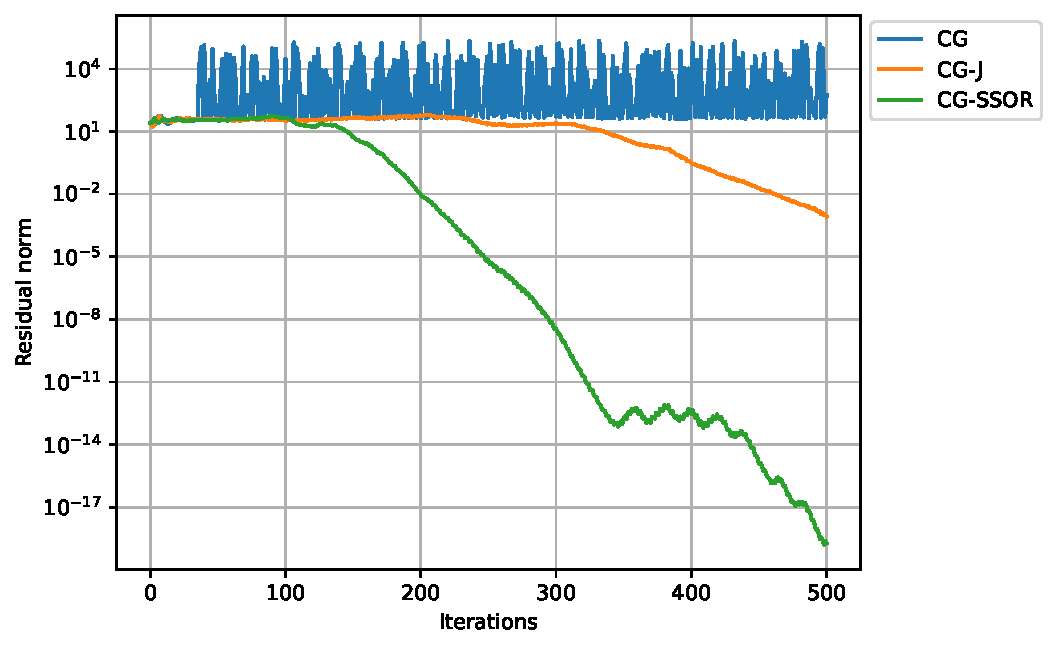
\includegraphics[width=\textwidth]{Figures/Results.pdf}
    \caption{Convergence of the Conjugate Gradient method with different preconditioners.}
    \label{fig:results}
\end{figure} 

As it's possible to see, the CG without a preconditioner did not converge to the solution. The Jacobi preconditioner improved the convergence and reached an error of $10^{-3}$ in 500 iterations. The SSOR preconditioner, however, was the most efficient, solving the system in 500 iterations with machine precision.

